% Name: Full adder
% Description: Two half adders and an OR gate adding A, B, and a carry in: the sum is A ⊕ B ⊕ Cᵢₙ and the carry out is AB + Cᵢₙ(A ⊕ B).
% Tags: full adder, logic gates, binary addition, arithmetic circuit

\usetikzlibrary{circuits.logic.US}

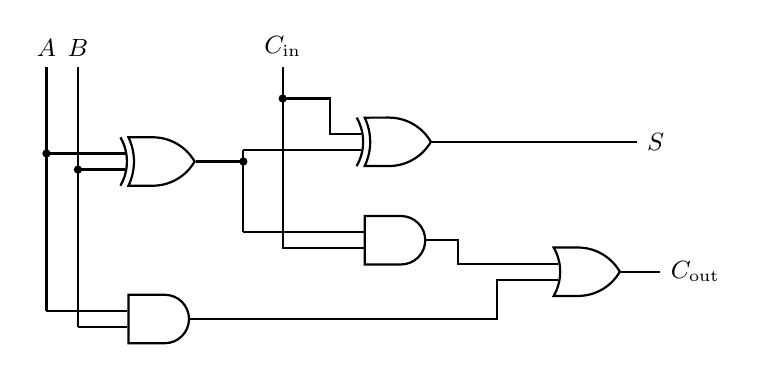
\begin{tikzpicture}[circuit logic US, thick, every circuit symbol/.style={thick}, every node/.style={font=\small}]
  \node[xor gate] (x1) at (2,2) {};
  \node[and gate] (a1) at (2,0) {};
  \node[xor gate] (x2) at (5,2.25) {};
  \node[and gate] (a2) at (5,1) {};
  \node[or gate] (o) at (7.4,0.6) {};
  % Input buses: A and B on the left, the carry in between the two stages
  \coordinate (A) at (0.6,0); \coordinate (B) at (1,0); \coordinate (C) at (3.6,0); \coordinate (M) at (3.1,0);
  \draw (x1.input 1) -- (x1.input 1 -| A) (a1.input 1) -- (a1.input 1 -| A);
  \draw (x1.input 2) -- (x1.input 2 -| B) (a1.input 2) -- (a1.input 2 -| B);
  \draw (A |- 0,3.2) node[above] {$A$} -- (a1.input 1 -| A) (B |- 0,3.2) node[above] {$B$} -- (a1.input 2 -| B);
  \fill (x1.input 1 -| A) circle (1.5pt) (x1.input 2 -| B) circle (1.5pt);
  \draw (x1.output) -- (x1.output -| M) (x2.input 2 -| M) -- (x2.input 2) (a2.input 1 -| M) -- (a2.input 1) (x2.input 2 -| M) -- (a2.input 1 -| M);
  \fill (x1.output -| M) circle (1.5pt);
  % The carry in joins the upper XOR through a jog, so its junction stays clear of the one wire that crosses it
  \draw (C |- 0,3.2) node[above] {$C_\mathrm{in}$} -- (a2.input 2 -| C) -- (a2.input 2) (C |- 0,2.8) -- (4.2,2.8) |- (x2.input 1);
  \fill (C |- 0,2.8) circle (1.5pt);
  \draw (a2.output) -- ++(0.4,0) |- (o.input 1);
  \draw (a1.output) -- ++(3.9,0) |- (o.input 2);
  \draw (x2.output) -- ++(2.6,0) node[right] {$S$};
  \draw (o.output) -- ++(0.5,0) node[right] {$C_\mathrm{out}$};
\end{tikzpicture}
